\subsection{Will I get the dukedom promised by the King?}
\begin{frame}[t]{Will I get the dukedom promised by the King?}
\begin{columns}[T, onlytextwidth]
\column{0.5\textwidth}
\Jupiter\ is L1, direct, in the 10th (most elevated planet) \\
\hspace{1em}\Sun\ \& \Venus\ $\Rightarrow$ \Square\ from \Sagittarius\ on 1st (received) \\
\hspace{1em}aspects both his domiciles \Sagittarius\ (1st) and \Pisces\ (4th) \\
\hspace{1em}aspects the 7th (connections to all 4 angles) \\
\hspace{1em}signifying he will get his dukedom\\
\vspace{0.5em}
\Mercury\ is L7, retro, a rebel opponent in the matter \\
\hspace{1em}cadent in the 12th \\
\hspace{1em}$\Rightarrow$ \Opposition\ \Saturn\ retro, cadent in 6th\footnotemark[1] (no reception) \\
\hspace{1em}dispositor, \Venus, is combust, worsening matters \\
\hspace{1em}indicates destruction for the opponent \\
\vspace{0.5em}
\Mercury\ retro, by transit, $\Rightarrow$ \Sextile\ \Jupiter\ with reception indicates the rebel opponent will end by seeking "peace and accommodation" from the querent

\column{0.5\textwidth}
\begin{center}
{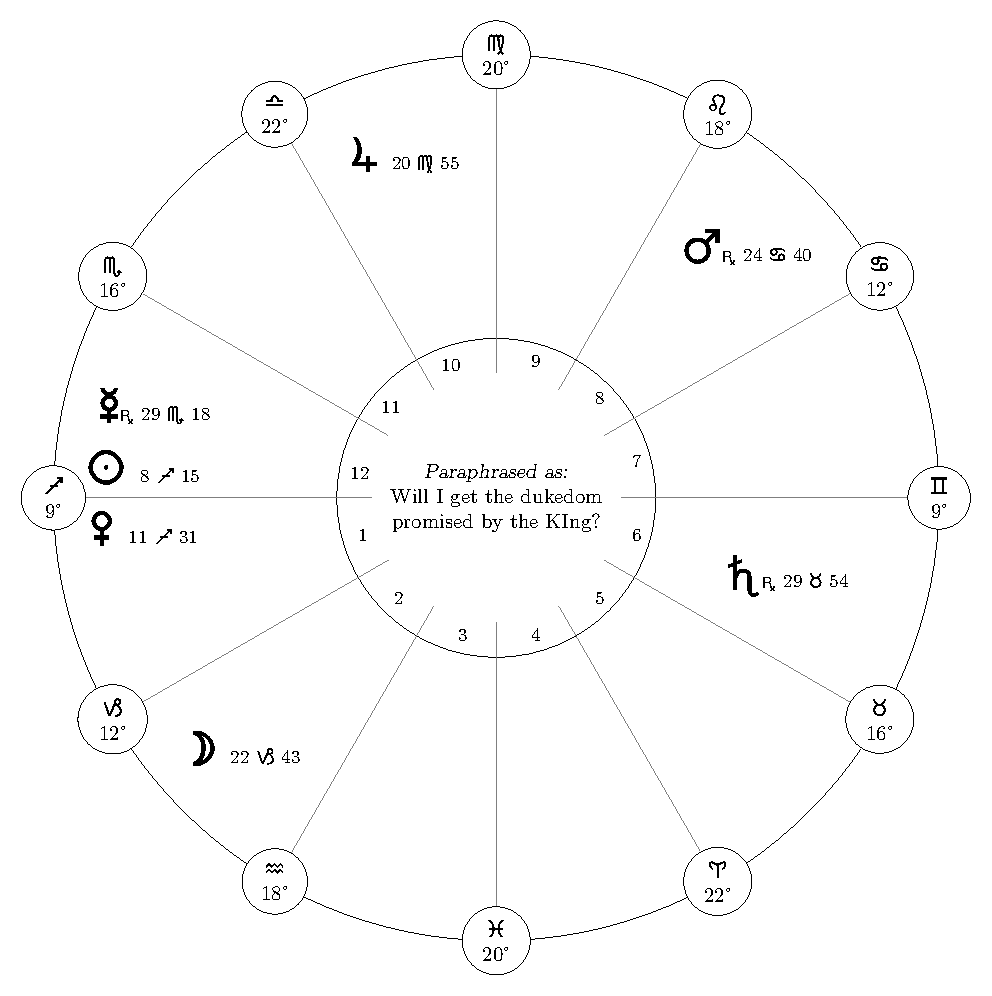
\includegraphics[width=0.9\textwidth]{charts/52-chart-dukedom}} \\
\scriptsize
The MC was not given, only the Asc degree. The other cusps are in the text Holden used but are not original to Masha'Allah.
\end{center}
\end{columns}
\footnotetext[1]{Hand notes this can only be true by Primary Direction.}

\end{frame}
% --------------------------------------------------------------
\begin{frame}[t]{Dukedom Chart as Battle Chart}
Masha'Allah goes further into the chart, reading it as a 'battle' or 'war' chart; he begins with the \Moon, using it's separating to identify the querent and its application to identify the rebel lord. \\
\vspace{0.25cm}
\Jupiter\ in \Virgo\ \Trine\ (not rec'd) $\Leftarrow$ \Moon\ in \Capricorn\ $\Rightarrow$ \Opposition\ \Mars\ in \Cancer\ (mixed reception) \\
\hspace{1em}\Moon\ is significator of the opponent  in the 2nd (support for querent) \\
\hspace{1em}\Mars\ retro, in 8th, in his Fall; indicating the opponents penury (8th is 2nd from 7th) \\
\hspace{1em} Masha'Allah says this indicates the rebel lord could not pay his army \\
\hspace{1em} so the querent bought them off; ending the battle \\
\vspace{0.25cm}
But, as \Mars\ is the dispositor of \Mercury\ (L7), and it is in a strong reception with the \Moon, the rebel lord will not lose everything and, as already noted, \Mercury's \Sextile\ to \Jupiter\ indicates a peaceful conclusion for all involved.



\end{frame}